\section{Comportement}
\label{sec:Comportement}
	Concernant les blessures préalablement observées lors du stage de B. SOMON, aucune n'a pu être à nouveau visualisée durant mon stage. Les animaux ont cependant été qualifiés de "plus sensible à leurs environnement que la normale" par les animaliers en charges de ceux-ci. On peut donc penser que durant le stage précédent, comme l'animalerie n'était pas la même, les animaux étaient soumis à un stress plus importants, et adoptaient en réponse à ce stress un comportement d'automutilation.

\section{Structure du cerveau}
\label{sec:NisslResultat}
	La coloration de Nissl, ici à base de Crésyl violet, est un marquage classique du tissu nerveux avec une molécule basique, qui marque particulièrement l'acide nucléique (\acrshort{adn} et \acrshort{arn}) des cellules car basophile (ces structures au microscope prennent le nom de "Corps de Nissl'). Ce marquage est important sur les neurones, riches en \gls{re} rugueux, et donc avec une grande quantité d'\acrshort{arn}. Cette coloration permet ainsi de mettre en évidence les motifs des différentes structures cellulaires au sein du tissu nerveux.

	Afin de visualiser si la mutation \mcrd altérait l'organisation structurale du cerveau, une coloration de Nissl a été réalisée sur 4 individus : 2 souris mutantes et 2 souris sauvages (1 mâle et 1 femelle pour chaque groupe) (\cref{fig:NisslResultat}). Ce marquage a permis de mettre en évidence que la mutation de \gls{musk} ne modifiait pas de manière visible l'organisation du cerveau, à la fois chez les souris femelles (\cref{fig:FemWTNissl,fig:FemMutNissl}) et mâles (\cref{fig:MaleWTNissl,fig:MaleMutNissl}). 

	\begin{figure}[h] %Figure Nissl Résultats
		\begin{center}
			\begin{subfigure}[h]{0.49\textwidth}%F437 WT Nissl 33 l2.tif
				\caption{}
				\label{fig:FemWTNissl}
				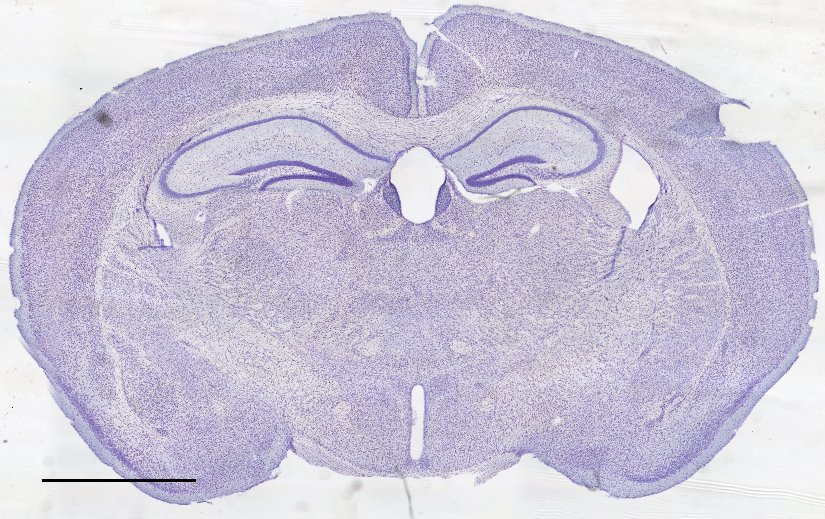
\includegraphics[width=\textwidth]{./Images/Nissl/FemWT.jpg}
			\end{subfigure}
			\begin{subfigure}[h]{0.49\textwidth}%F435 Mut Nissl 38.tif
				\caption{}
				\label{fig:FemMutNissl}
				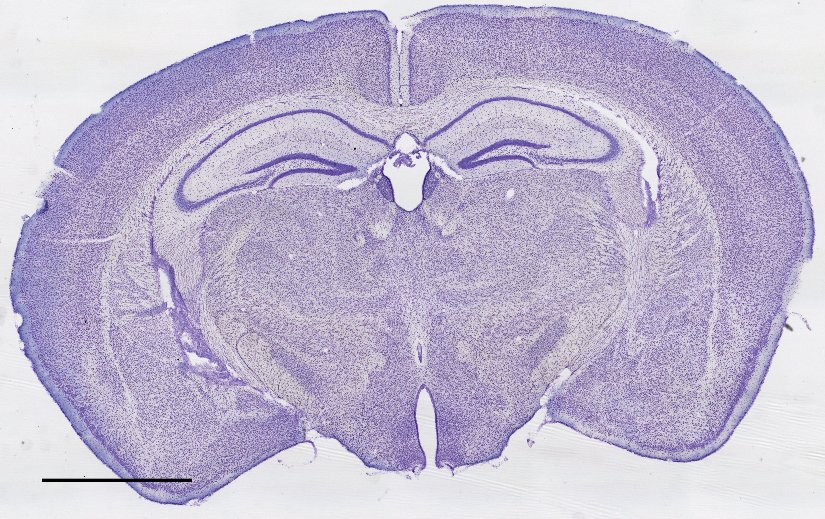
\includegraphics[width=\textwidth]{./Images/Nissl/FemMut.jpg}
			\end{subfigure}
			\begin{subfigure}[h]{0.49\textwidth}%M2 WT Nissl #031.tif
				\caption{}
				\label{fig:MaleWTNissl}
				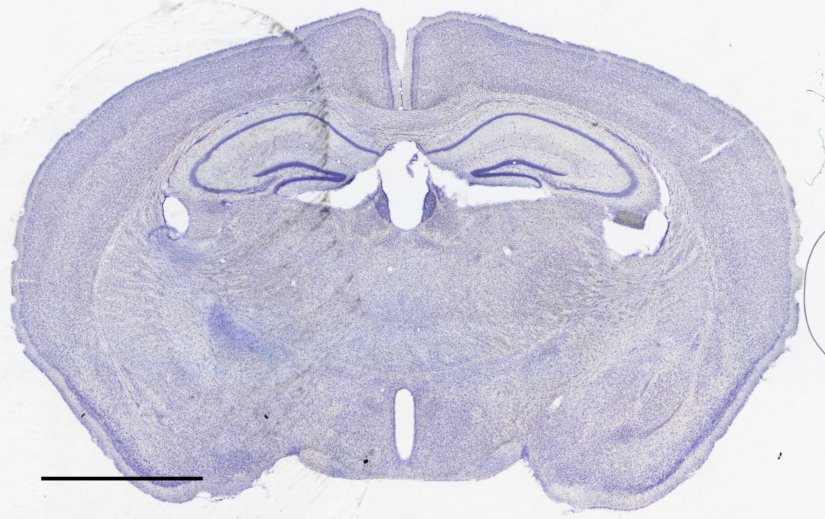
\includegraphics[width=\textwidth]{./Images/Nissl/MaleWT.jpg}
			\end{subfigure}
			\begin{subfigure}[h]{0.49\textwidth}%M442 Mut Nissl lame 3 36.tif
				\caption{}
				\label{fig:MaleMutNissl}
				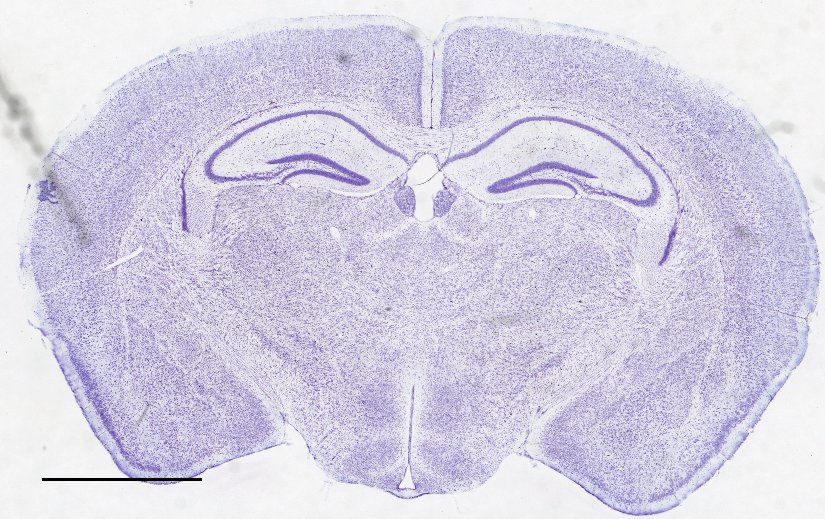
\includegraphics[width=\textwidth]{./Images/Nissl/MaleMut.jpg}
			\end{subfigure}
		\end{center}
		\caption{Pas de modifications structurelles observées chez les mutants.}
		\descfig{Coloration de Nissl sur : \subref{fig:FemWTNissl} Femelle sauvage, \subref{fig:FemMutNissl} Femelle mutante, \subref{fig:MaleWTNissl} Mâle sauvage, \subref{fig:MaleMutNissl} Mâle mutant. Images représentatives de coupes réalisées au niveau de l'hippocampe. Âge moyen des souris : 30 jours. Barre d'échelle : 2 mm.}
		\label{fig:NisslResultat}
	\end{figure}
	%\FloatBarrier

\section{Immunomarquage}
\label{sec:IHC}

	\subsection{\acrshort{neun}}
	\label{ssec:neun}
	\Acrshort{neun} est un marqueur du  corps cellulaire et des noyaux de presque tout les neurones, couramment utilisé \cite{Guselnikova2015}. Ce marquage à été utilisé afin de vérifier la distribution et le nombre des neurones au niveau de l'hippocampe des souris \mcrd était perturbée ou non.
	
	\subsection{\acrshort{musk} et \acrshort{gfap}}
	\label{ssec:musk}
	Après avoir observé l'organisation neuronale du cerveau de souris, j'ai voulu observé les régions du cerveau qui exprimaient \gls{musk}. Pour cela, j'ai eu recours à des techniques d'immunomarquages. L'anticorps utilisé est un anticorps polyclonal de lapin, ayant comme immunogène pour sa création un protéine recombinante du domaine extracellulaire de \gls{musk}.
	
	Malgré le fait que le niveau d'expression de \gls{musk} soit considéré comme faible dans le tissu nerveux, j'ai quand même pu observé un marquage de cette protéine dans diverses régions discrètes du cerveau : Hippocampe (couche radiaire et moléculaire principalement), Corps calleux, Habenula, Fasciculus retroflexus, Capsule interne, Noyau caudé, 3ème ventricule ventrale, Cervelet principalement. \todo{fig avec schéma localisation ?}.
	
	Dans ces régions, le marquage prenait la forme de prolongement cellulaires, qui rappelait ce que l'on peut observer après marquage d'astrocytes. Afin d'étudier cette hypothèse, un co-marquage entre \gls{musk} et \acrshort{gfap}, un marqueur des astrocytes a été réalisé.
	
	Pour réaliser le marquage de \acrshort{gfap}, deux anticorps différents ont été utilisés. Le premier, fourni d'abord par l'équipe de C. AGULHON, provient de chez Millipore-Merck (\cref{table:Ac}, réf. MAB360) et fonctionne correctement. Le second anticorps, provenant de chez Abcam (\cref{table:Ac}, réf. ab4648) et commandé suite à une indisponibilité du premier anticorps, s'est révélé inefficace à différentes concentrations testées ($1{:}100$, $1{:}50$). Le premier anticorps a put heureusement être à nouveau commandé pour la suite des expériences.
	
	Cependant, le marquage observé de \gls{musk} ne ressemble pas à ce que l'on peut observer au niveau de la \gls{jnm}.  On peut donc émettre un doute sur la spécificité du marquage. Comme il n'existe pas vraiment d'autres anticorps dirigés contre \gls{musk} utilisables en \gls{ihc}, j'ai dû essayé d'autres moyen afin de tenter de confirmer la spécificité du marquage. Tout d'abord, un co-marquage \gls{musk}/\acrshort{gfap} à été réalisé sur des sections de cerveau d'embryon de souris \gls{musk} KO (stade E18.5), la mutation étant létale après la naissance pour cause de défaillance respiratoire. Aucun marquage de \gls{musk} ni de \acrshort{gfap} n'est cependant observé. Pour tenter alors de montrer la présence de \gls{musk} dans le cerveau, une immunoprécipitation est envisagée.
	
	(Voir si anticorps Abcam ab58697 ab218245 ab5510 ab92950 ab228488 ont été testés.)

\section{Immunoprécipitation}
\label{sec:IPresultat}
	Afin de confirmer la détection de \gls{musk} dans diverse région du cerveau, une immunoprécipitation suivie d'un \gls{wb} a été réalisée sur trois structures : l'hippocampe, le cervelet et le cortex de trois souris C57Bl/6 sauvage. Un \gls{wb} de \gls{musk} a déjà été décrit sur des diverses structures du cerveau \cite{Garcia-Osta2006}, mais à partir d'extrait total. Durant son stage, B. SOMON a tenté de réaliser un \gls{ip} suivi d'un \gls{wb}, mais sans obtenir de résultats probant. Ici, la principale modification apportée au protocole précédemment utilisée par cette étudiante est l'utilisation de tampon RIPA (adjonction de déoxycholate de sodium et de \acrshort{sds} dans le tampon) qui permet une meilleure lyse et une meilleure préservation des protéines lors de l'extraction.
	
	Afin de vérifier si la technique fonctionnait, j'ai tout d'abord prélevé l'hippocampe, le cervelet et le cortex de trois souris C57Bl/6 puis réalisé une \gls{ip} de \gls{musk} dessus, qui a ensuite été migré dans un gel pour un \gls{wb}. Surprenamment, des bandes de taille attendue (110kDa) ont été révélée dans l'hippocampe et le cervelet, alors que dans le cortex, une bande d'intensité plus faible semblait être présente, ce qui pourrait correspondre au fait que dans cette région du cerveau, je ne vois pas de marquage de \gls{musk} (\cref{fig:WBbon}). Cependant, comme la taille des bandes ne correspondaient pas tout à fait à celle du témoin positif (extrait de cellules transfectées HEK293, à 130kDa), l'expérience à été refaite avec des souris \mcrd et sauvages, issues de la même lignée. En effet, suite à la mutation, la protéine \gls{musk} à un poids moléculaire de ~80kDa : si c'est bien \gls{musk} qui est détécté, on devrait alors avoir un décalage entre les individus. Cette fois-ci cependant, l'expérience ne s'est pas montrée concluante, rien n'a été révélé (gel non montré). Afin de confirmer ce résultat, l'expérience a finalement été tentée une troisième fois avec comme témoin positif les extraits protéiques de la première expérience (cervelet et cortex, plus assez d'extraits d'hippocampe pour recommencer). Cette fois encore, rien n'a été révélé (\cref{fig:WBpasbon}).
		
	\begin{figure}[h]
		\begin{center}
			\begin{subfigure}[h]{0.49\textwidth}
				\caption{}
				\label{fig:WBbon}
				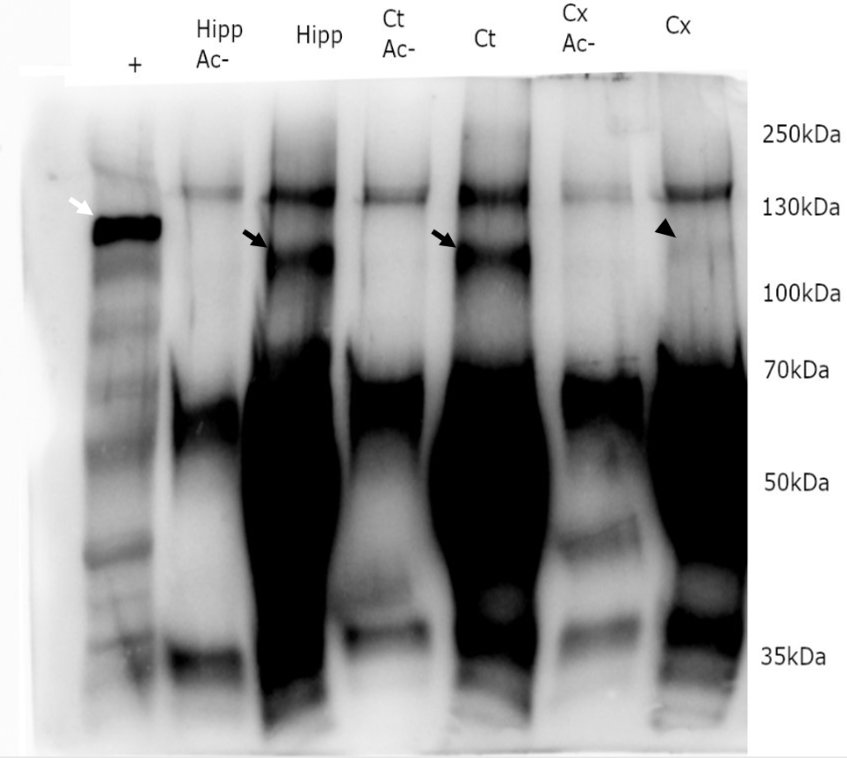
\includegraphics[width=\textwidth]{./Images/WB/2018-04-09.jpg}
			\end{subfigure}
			\begin{subfigure}[h]{0.49\textwidth}
				\caption{}
				\label{fig:WBpasbon}
				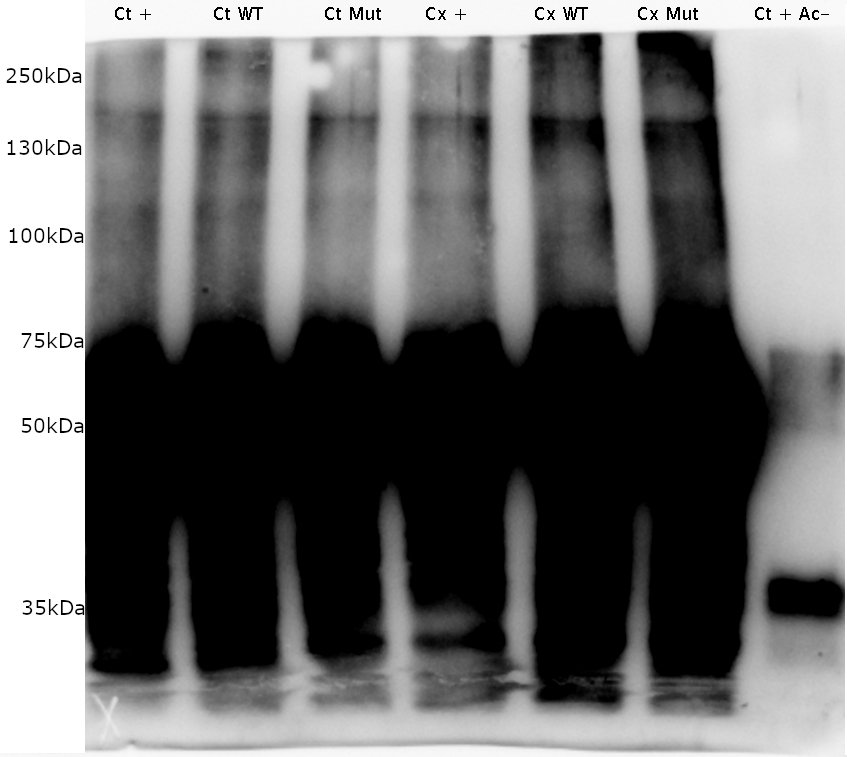
\includegraphics[width=\textwidth]{./Images/WB/2018-05-03.jpg}
			\end{subfigure}
		\end{center}
		\caption{Une \gls{ip} ne permet pas de confirmer la présence de \gls{musk} dans différentes parties du cerveau.}
		\descfig{%
			\subref{fig:WBbon} : \gls{ip} suivie de \gls{wb} sur 3 souris C57BL/6. Des bandes sont révélés aux alentours de 110kDa pour les régions de l'hippocampe et du cervelet (flèches noires). Une bande de faible intensité semble être présente pour le cortex (tête de flèche noire). Témoin positif : 15µL d'extrait cellulaire de cellules HEK293 transfectées, bande à 130kDa (flèche blanche). %
			\subref{fig:WBpasbon} : \gls{ip} suivie de \gls{wb} sur 3 souris \mcrd (Mut) et 3 souris sauvages (WT) issues de la même souche. Aucune bande n'est révélée, avec ou sans anticorps durant \gls{ip}. Rien n'est révélé non plus chez le témoin positif : Extrait de cervelet et cortex issus de la première expérience. Hipp : Hippocampe, Ct : Cervelet, Cx : Cortex, + : Témoin positif, Ac- : Sans anticorps lors de l'\gls{ip}, Mut : Mutant, \acrshort{wt} : Sauvage. Poids moléculaire de \gls{musk} attendu : 110kDa.
		}
		\label{fig:WBResultat}
	\end{figure}

\section{Expression de \gls{musk}}
\label{sec:ExpressionMuSK}
	Il est intéressant de connaître le niveau d'expression de la protéine \gls{musk} dans le cerveau, afin de voir si la mutation allait impactée l'expression de la protéine. Pour cela, j'ai eu recours à la technique de \gls{qpcr} sur trois structures différentes : le cervelet, et l'hippocampe gauche ou droit. En effet, des résultats très préliminaire dans le laboratoire chez des 2 souris de souche C57Bl/6 (1 mâle et 1 femelle) avait montrée une légère différence d'expression selon le coté du cerveau étudié. De plus, on retrouvait également une différence entre des individus de sexe opposé. Il était donc nécessaire de reprendre cette technique chez un plus grand nombre d'animaux afin de confirmer ou non ces tendances.
